
\documentclass{article}
\usepackage{amsmath}
\usepackage{graphicx}
\usepackage{subcaption}
\usepackage{array}

\begin{document}

\begin{titlepage}
  \centering
  \vspace*{2cm}
  {\Huge\bfseries Report\par}
  \vspace{2cm}
  {\Large\itshape Homework 1\par}
  \vspace{0.5cm}
  {\large\itshape Goal: Develop models for 10-class classification problems with medium and large input space\par}
  \vfill
  {\Large Andrea Massignan\par}
  {\Large 1796802\par}
  \vfill
  {\large\today\par}
\end{titlepage}

\begin{titlepage}

  \section*{Project Overview}

  The goal is to provide two different solution for a 10-class classification problem.

  \section{Dataset}

  The datasets used in this project consists in training sets and blind test sets.
  The training sets are composed by 50000 samples, each one with 100 features for Dataset 1 and 1000 features for Dataset 2.
  The blind test sets are composed by 10000 samples, each one with 100 features for Dataset 1 and 1000 features for Dataset 2.
  The labels are 10, one for each class.

  \begin{itemize}
    \item \texttt{X\_train}: 50000 samples for each dataset.
    \item \texttt{n\_features}: 100 for Dataset 1 and 1000 for Dataset 2.

  \end{itemize}

  \section{Data Exploration}
  The datasets, that are in a csv file, the elements $V^{(i)}$ belonging
  to the $X$ column are feature vectors that represent the input data.
  \newline
  \newline
  The Y column contains the associated labels $C_k$(k=0,...9).
  \newline
  \newline
  Thus, each line i in column X is a feature vector structured as:
  \newline
  \newline
  [$V^{(i)}_1$, $V^{(i)}_2$, ..., $V^{(i)}_j$, ... , $V^{(i)}_d$]
  \newline
  \newline
  Where d is the size of the feature vector with sizes described before.
  \newline
  \newline
  And $i=1,...,n$, where n is the number of samples in the dataset as specified before.
  \newline
  \newline
  These are loaded with an helper function called \texttt{load\_data} that returns the training set in the X matrix and the labels in the Y vector.
  \newline
  \newline
  Then the training set is split into \texttt{X\_train} and \texttt{Y\_train} with a test size of $0.2$ and different random states.
  \newline
  \newline
  Since the dataset is already vectorized, no further preprocessing is needed at the moment.

  \section{Metrics}
  The metrics used to evaluate the models are the accuracy and the confusion matrix.
  \newline

  \subsection{Precision}
  Precision is a measure of the accuracy of the positive predictions made by a model. It is the ratio of true positive predictions to the total number of positive predictions made by the model (both true positives and false positives). Precision is calculated using the formula:
  \[
    \text{Precision} = \frac{\text{True Positives}}{\text{True Positives + False Positives}}
  \]
  Precision provides insight into the model's ability to avoid making false positive predictions. A high precision indicates that when the model predicts a positive class, it is likely to be correct.

  \subsection{Recall (Sensitivity or True Positive Rate)}
  Recall measures the ability of a model to correctly identify all relevant instances of the positive class. It is the ratio of true positive predictions to the total number of actual positive instances in the dataset (including both true positives and false negatives). Recall is calculated using the formula:
  \[
    \text{Recall} = \frac{\text{True Positives}}{\text{True Positives + False Negatives}}
  \]
  Recall is especially important when the cost of false negatives (missing a positive instance) is high, as it focuses on minimizing false negatives.

  \subsection{F1-Score}
  The F1-score is the harmonic mean of precision and recall. It provides a balanced measure that considers both false positives and false negatives. The F1-score is calculated using the formula:
  \[
    \text{F1-Score} = \frac{2 \times \text{Precision} \times \text{Recall}}{\text{Precision + Recall}}
  \]
  F1-score is useful when there is an uneven class distribution or when false positives and false negatives have different consequences.

  \subsection{Support}
  Support refers to the number of actual instances of each class in the dataset. It is the count of true positive and true negative instances for each class. Support is not directly involved in the calculation of precision, recall, or F1-score, but it provides context by showing how many instances belong to each class.

  \begin{center}
    {\Huge\bfseries Classification\par}
  \end{center}
  \vspace{2cm}

  \section{Data Loading and Splitting}

  \subsection{Loading Dataset 1}
  The data loading process begins with dataset 1, where the feature matrix \(X\) and label vector \(Y\) are extracted using the \texttt{load\_data} function. An informative message is printed to indicate the commencement of this operation. The resulting shape of matrix \(X\) is then presented, providing insights into the number of samples and features within dataset 1.

  \subsection{Loading Dataset 2}
  An analogous procedure is employed for dataset 2. The feature matrix \(X2\) and label vector \(Y2\) are obtained through the \texttt{load\_data} function. A corresponding message is printed, and the shape of \(X2\) is displayed to convey the dataset's sample and feature dimensions.

  \subsection{Splitting Data}
  The subsequent steps involve splitting the loaded data into training and testing sets:

  \begin{verbatim}
  X_train1, X_test1, Y_train1, Y_test1 = train_test_split(X, Y, ...)
    ...
  X_train4, X_test4, Y_train4, Y_test4 = train_test_split(X2, Y2, ...)
  \end{verbatim}

  Utilizing the \texttt{train\_test\_split} function, both dataset 1 and dataset 2 are partitioned into training and testing sets. Each dataset undergoes this process twice, resulting in four sets per dataset.
  The \texttt{test\_size} parameter dictates the proportion allocated for testing (20\%), while \texttt{random\_state} ensures reproducibility.
  \newline
  \newline
  The code concludes by acknowledging the completion of data loading and splitting.
  \newline
  \newline
  The resulting variables (\(X\_train1\), \(X\_test1\), \(Y\_train1\), \(Y\_test1\), etc.) are now ready for subsequent machine learning tasks.

  \section*{First Evaluation with Binary Classification}
  After the data is loaded and splitted, the user is prompted to choose which of the dataset to use and then what type of model to use for the classification task. The user can choose between:
  \section{Bernoulli}
  BernoulliNB is a Naive Bayes classifier specifically tailored for multivariate Bernoulli models. Similar to MultinomialNB, this classifier is well-suited for handling discrete data.
  \newline
  \newline
  The key distinction lies in their data types:
  MultinomialNB deals with occurrence counts, while BernoulliNB is optimized for binary or boolean features.
  BernoulliNB is preferred over other Naive Bayes classifiers when dealing with datasets where features are binary or boolean.
  \newline
  \newline
  It is well-suited for problems involving discrete, binary decision-making based on the presence or absence of features.
  Additionally, BernoulliNB is a simpler model with fewer parameters, making it advantageous for scenarios with limited training data and leading to faster training and prediction times.

  \subsection{Classification}
  Overall the model performs well, with an average accuracy of 90\%, however class 3 has a lower recall of 71\%, meaning that the model struggles to capture all instances of the class.
  \newline
  \newline
  Even class 4 has a lower precision of 78\%, meaning that when the model predicts this class it's not always correct.

  \begin{figure}[htbp]
    \centering
    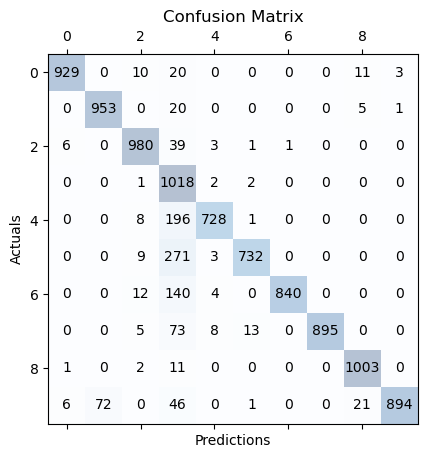
\includegraphics[width=0.4\textwidth]{bernoulliCM.png}
    \caption{Confusion Matrix for BernoulliNB}
    \label{fig:sample}
  \end{figure}

  \section{SVM}
  Support Vector Machine is a supervised machine learning algorithm used for classification and regression tasks. It's particularly powerful in high-dimensional spaces and is effective in cases where the margin between different classes is clear.
  \newline
  \newline
  The SVM model performs well in terms of precision and recall for most classes, but there are variations across different digits.
  \newline
  In this particular case we are using a linear kernel, which is a good choice for high-dimensional data, however, it may not be the best choice for this particular dataset.

  \begin{itemize}
    \item The accuracy is around 83\% which is lower than the BernoulliNB model.
    \item Some classes, like class 5, have lower support (973), while others, like class 7, have higher support (1048).
    \item The F1-scores are generally high, however, class 2 stands out with a lower F1-score (0.22).
    \item Notably, class 5 has a recall of 1.00, on the other hand, classes 2 and 3 have lower recall values.
    \item For most classes, precision is relatively high, however, there are exceptions, such as class 5, where precision is notably lower (0.40).
  \end{itemize}

  The lower performance in certain classes, especially in terms of recall for classes 2 and 3, indicates areas where the model may benefit from further improvement.

  \begin{figure}[htbp]
    \centering
    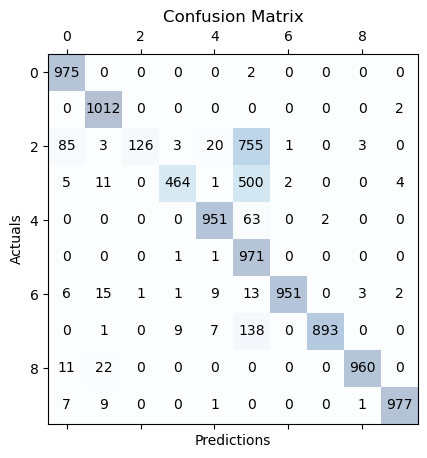
\includegraphics[width=0.5\textwidth]{SVMCM.png}
    \caption{Confusion Matrix for SVM}
    \label{fig:sample2}
  \end{figure}

  \section{Logistic Regression}
  Logistic regression is a statistical model that in its basic form uses a logistic function to model a binary dependent variable, although many more complex extensions exist. In regression analysis, logistic regression is estimating the parameters of a logistic model.
  \newline
  \newline
  The model has a small problem of never converging and thus never stopping the training, however, it still performs well in terms of accuracy, precision and recall.

  \begin{itemize}
    \item Overall accuracy is 98\%, indicating that the model correctly predicts the class labels for 98\% of the instances in the dataset.
    \item High F1-scores (close to 1.0) indicate a good balance between precision and recall, this means that the model is robust enough.
    \item High recall values (close to 1.0) indicate that the model captures a high percentage of actual positive instances, which is fine.
    \item Precision also is close to 1.0, meaning that the model has low false positive rate.
  \end{itemize}

  The model performs very well across various metrics, indicating its effectiveness in classifying instances in the given dataset.
  \newline
  \newline

  \begin{figure}[htbp]
    \centering
    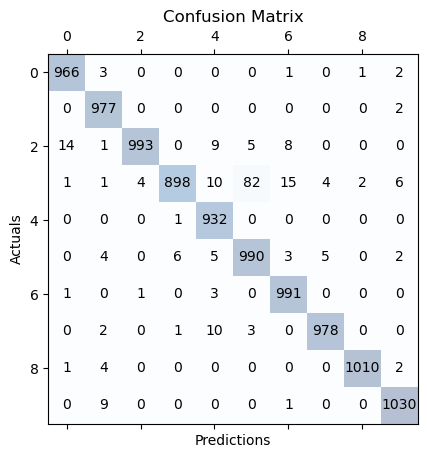
\includegraphics[width=0.55\textwidth]{LRCM.png}
    \caption{Confusion Matrix for Logistic Regression}
    \label{fig:sample3}
  \end{figure}

  \section*{Second Evaluation with Multiclass Classification}
  In this second batch we are using the same models as before, but with a different approach to the data.

  \section{Bernoulli to MultinomialNB}
  The Bernoulli model was almost fine, but still we want to improve the accuracy of the model, so we are going to use a MultinomialNB model with a multiclass approach.

  \begin{itemize}
    \item The accuracy is around 98\% which is better than the BernoulliNB model.
    \item Even the F1-scores are generally high, with a minimum of 0.96, better than the BernoulliNB model (minimum of 0.71).
    \item Recall is also higher, with a minimum of 0.94, better than the BernoulliNB model (minimum of 0.72).
    \item Precision is higher too, with a minimum of 0.94, better than the BernoulliNB model (minimum of 0.56).
  \end{itemize}

  The MultinomialNB model appears to be better suited for the given dataset, providing higher accuracy and more balanced precision-recall trade-offs across all classes compared to the BernoulliNB model.
  \newline
  \newline

  \begin{figure}[htbp]
    \centering
    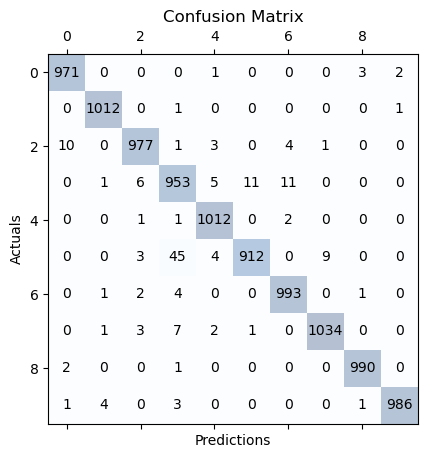
\includegraphics[width=0.55\textwidth]{MNCM.png}
    \caption{Confusion Matrix for MultinomialNB}
    \label{fig:sample4}
  \end{figure}

  \section{SVM}
  The SVM was perfoming well, but I want to give a slight modification to the hyperparameters, so I'm going to use polynomial kernel instead of linear.
  \newline
  \newline
  The model seems to performs better this way, in detail:

  \begin{itemize}
    \item The accuracy is around 99\%, way better than the 83\% of the linear kernel.
    \item The recall, precision and F1-scores are better too, with a minimum of 0.96, 0.97 and 0.97 respectively.
    \item Support values remain consistent, indicating that the number of instances for each class in the dataset is not significantly affected by the change in the kernel.
  \end{itemize}

  Overall the SVM with a poly kernel achieves a higher performance than the previous one ($linear$) and seems to be better suited for this type of dataset.
  \newline
  \newline

  \begin{figure}[htbp]
    \centering
    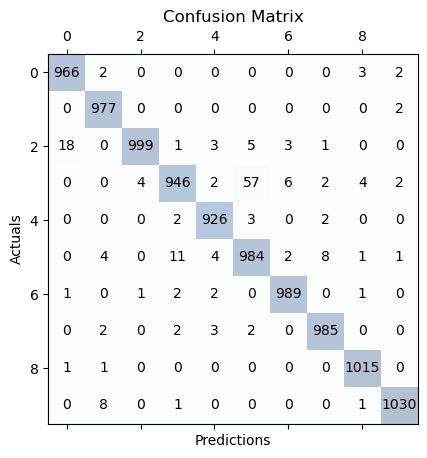
\includegraphics[width=0.58\textwidth]{SVM2CM.png}
    \caption{Confusion Matrix for SVM with poly kernel}
    \label{fig:sample5}
  \end{figure}

  \newpage

  \section{Logistic Regression}
  The Logistic Regression actually performed well even if it didn't converge, so I'm going to use the same model but with a different solver, to see if there could be any improvement.

  \begin{itemize}
    \item Tried the $newton$-$cg$ solver, it converged but gave a lower performance: accuracy of 0.88, recall of 0.84, precision of 0.86 and f1-score of 0.86.
    \item Tried the $sag$ solver, it gave a similar performance if slightly worse.
    \item Tried the $newton$-$cholesky$ solver, it converged but the result was similar to the $newton-cg$ solver: accuracy of 0.86, recall of 0.83, precision of 0.94 and f1-score of 0.84.
    \item Tried the $liblinear$ solver, it converged but the result was still worse than the $saga$ solver: accuracy of 0.86, recall of 0.84, precision of 0.92 and f1-score of 0.85.
    \item Lastly the $lbfgs$ solver, it converged but the result was medium: accuracy of 0.89, recall of 0.90, precision of 0.95 and f1-score of 0.89.
  \end{itemize}

  The Logistic Regression model with the $saga$ solver still seems to be the best choice.

  \begin{figure}[htbp]
    \centering
    \begin{subfigure}[t]{0.3\linewidth}
      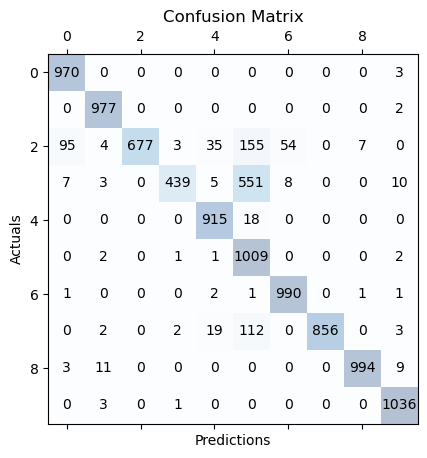
\includegraphics[width=\linewidth]{LRMC(lbfgs).png}
      \caption{$lbfgs$ solver}
      \label{fig:sample6a}
    \end{subfigure}
    \hfill
    \begin{subfigure}[t]{0.3\linewidth}
      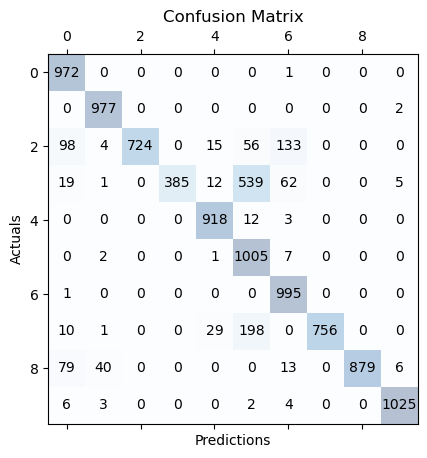
\includegraphics[width=\linewidth]{LRMC(liblinear).png}
      \caption{$liblinear$ solver}
      \label{fig:sample6b}
    \end{subfigure}
    \hfill
    \begin{subfigure}[t]{0.3\linewidth}
      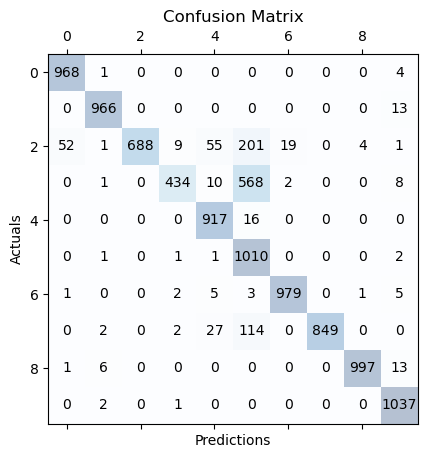
\includegraphics[width=\linewidth]{LRMC(newton-cg).png}
      \caption{$newton$-$cg$ solver}
      \label{fig:sample6c}
    \end{subfigure}
    \hfill
    \begin{subfigure}[t]{0.3\linewidth}
      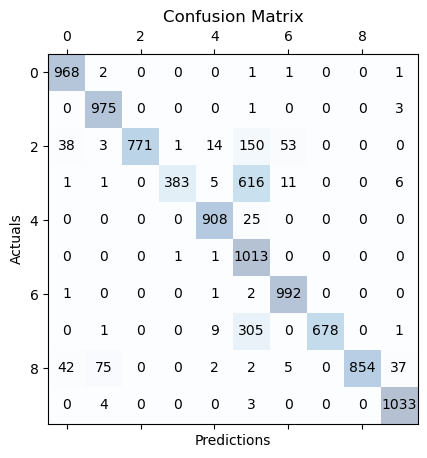
\includegraphics[width=\linewidth]{LRMC(newton-cholesky).png}
      \caption{$newton$-$cholesky$ solver}
      \label{fig:sample6d}
    \end{subfigure}
    \hfill
    \begin{subfigure}[t]{0.3\linewidth}
      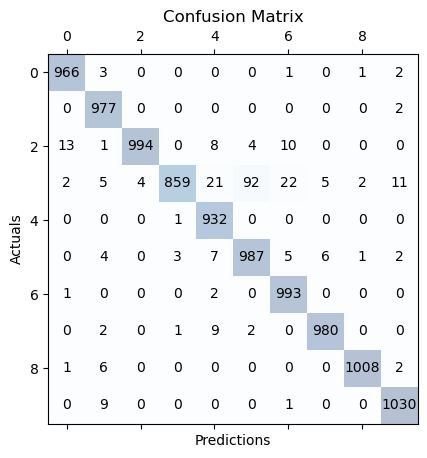
\includegraphics[width=\linewidth]{LRMC(sag).png}
      \caption{$sag$ solver}
      \label{fig:sample6f}
    \end{subfigure}
  \end{figure}

  \section*{Blind Tests}
  We were provided with blind tests in the format of csv files that are structured as follows:
  \newline
  \newline

  \begin{table}[htbp]
    \centering
    \begin{tabular}{|c|>{\centering\arraybackslash}m{8cm}|}
      \hline
      Index & X \\
      \hline
      % Add your data here
      0 & [$V^{(0)}_1$, $V^{(0)}_2$, ..., $V^{(0)}_j$, ... , $V^{(0)}_d$] \\
      \hline
      \dots & \dots \\
      \hline
      i & [$V^{(i)}_1$, $V^{(i)}_2$, ..., $V^{(i)}_j$, ... , $V^{(i)}_d$] \\
      \hline
      \dots & \dots \\
      \hline
      N & [$V^{(N)}_1$, $V^{(N)}_2$, ..., $V^{(N)}_j$, ... , $V^{(N)}_d$] \\
      \hline
    \end{tabular}
    \label{tab:sample}
  \end{table}

  The blind test structure consists of a two-column table with "Index" and "X." The "Index" column ranges from 0 to N, representing the index of each feature vector. The "X" column contains feature vectors denoted as arrays [Vij] with elements Vij, where "i" is the index and "j" ranges from 1 to d, representing features. This format signifies N samples, each with a feature vector of length d.
  \newline
  \newline

  \section{Predictions}
  The predictions are made using the best model for each dataset, the results are the following:

  \begin{itemize}
    \item BernoulliNB: [3 8 8 ... 5 1 7]
    \item SVM with linear kernel: [5 8 8 ... 5 1 7]
    \item Logistic Regression: [3 8 8 ... 5 1 7]
    \item MultinomialNB: [3 8 8 ... 5 1 7]
    \item SVM with poly kernel: [3 8 8 ... 5 1 7]
    \item Logistic Regression with multiclass: [3 8 8 ... 5 1 7]
  \end{itemize}

  The predictions are saved in two csv files, one for each database.

\end{titlepage}


\end{document}
